\documentclass[10pt,a4paper,onecolumn]{article}
% \usepackage[utf8]{inputenc}
\usepackage{marginnote}
\usepackage{graphicx}
\usepackage{xcolor}
\usepackage{authblk,etoolbox}
\usepackage{titlesec}
\usepackage{calc}
\usepackage{hyperref}
\hypersetup{breaklinks=true,
            bookmarks=true,
            pdfauthor=
{
      Pamela Hathway,
      Dan F. M. Goodman,,
  },
            pdftitle=
{
[Re] Spike Timing Dependent Plasticity Finds the Start of Repeating Patterns
in Continuous Spike Trains
},
            colorlinks=true,
            citecolor=blue,
            urlcolor=blue,
            linkcolor=blue,
            pdfborder={0 0 0}}
\urlstyle{same}
\usepackage{tcolorbox}
\usepackage{ragged2e}
\usepackage{fontspec}
%\defaultfontfeatures{Path = /usr/local/texlive/2018/texmf-dist/fonts/opentype/public/fontawesome/}
\usepackage{fontawesome}
\usepackage{caption}
\usepackage{listings}
\lstnewenvironment{code}{\lstset{language=Haskell,basicstyle=\small\ttfamily}}{}



%\usepackage{fancyvrb}
%\VerbatimFootnotes
%\usepackage{graphicx}
%\usepackage{mdframed}
%\newmdenv[backgroundcolor=lightgray]{Shaded}


\usepackage{longtable,booktabs}

\usepackage[
  backend=biber,
%  style=alphabetic,
%  citestyle=numeric
]{biblatex}
\bibliography{bibliography.bib}



% --- Macros ------------------------------------------------------------------
\renewcommand*{\bibfont}{\small \sffamily}

\definecolor{red}{HTML}{CF232B}
\newcommand{\ReScience}{Re{\bfseries \textcolor{red}{Science}}}

\newtcolorbox{rebox}
   {colback=blue!5!white, colframe=blue!40!white,
     boxrule=0.5pt, arc=2pt, fonttitle=\sffamily\scshape\bfseries,
     left=6pt, right=20pt, top=6pt, bottom=6pt}

\newtcolorbox{repobox}
   {colback=red, colframe=red!75!black,
     boxrule=0.5pt, arc=2pt, left=6pt, right=6pt, top=3pt, bottom=3pt}

% fix for pandoc 1.14     
\newcommand{\tightlist}{%
  \setlength{\itemsep}{1pt}\setlength{\parskip}{0pt}\setlength{\parsep}{0pt}}

% --- Style -------------------------------------------------------------------
\renewcommand*{\bibfont}{\small \sffamily}
\renewcommand{\captionfont}{\small\sffamily}
\renewcommand{\captionlabelfont}{\bfseries}

\makeatletter
\renewcommand\@biblabel[1]{{\bf #1.}}
\makeatother

% --- Page layout -------------------------------------------------------------
\usepackage[top=3.5cm, bottom=3cm, right=1.5cm, left=1.5cm,
            headheight=2.2cm, reversemp, includemp, marginparwidth=4.5cm]{geometry}

% --- Section/SubSection/SubSubSection ----------------------------------------
\titleformat{\section}
  {\normalfont\sffamily\Large\bfseries}
  {}{0pt}{}
\titleformat{\subsection}
  {\normalfont\sffamily\large\bfseries}
  {}{0pt}{}
\titleformat{\subsubsection}
  {\normalfont\sffamily\bfseries}
  {}{0pt}{}
\titleformat*{\paragraph}
  {\sffamily\normalsize}


% --- Header / Footer ---------------------------------------------------------
\usepackage{fancyhdr}
\pagestyle{fancy}
%\renewcommand{\headrulewidth}{0.50pt}
\renewcommand{\headrulewidth}{0pt}
\fancyhead[L]{\hspace{-1cm}
\includegraphics[width=4.0cm]{rescience-logo.pdf}}
\fancyhead[C]{}
\fancyhead[R]{} 
\renewcommand{\footrulewidth}{0.25pt}

\fancyfoot[L]{\hypersetup{urlcolor=red}
              \sffamily \ReScience~$\vert$
              \href{http://rescience.github.io}{rescience.github.io}
              \hypersetup{urlcolor=blue}}
\fancyfoot[C]{\sffamily 1 - \thepage}
\fancyfoot[R]{\sffamily Sep 2015 $\vert$
                        Volume \textbf{1} $\vert$
                        Issue \textbf{1}}
\pagestyle{fancy}
\makeatletter
\let\ps@plain\ps@fancy
\fancyheadoffset[L]{4.5cm}
\fancyfootoffset[L]{4.5cm}

% --- Title / Authors ---------------------------------------------------------
% patch \maketitle so that it doesn't center
\patchcmd{\@maketitle}{center}{flushleft}{}{}
\patchcmd{\@maketitle}{center}{flushleft}{}{}
% patch \maketitle so that the font size for the title is normal
\patchcmd{\@maketitle}{\LARGE}{\LARGE\sffamily}{}{}
% patch the patch by authblk so that the author block is flush left
\def\maketitle{{%
  \renewenvironment{tabular}[2][]
    {\begin{flushleft}}
    {\end{flushleft}}
  \AB@maketitle}}
\makeatletter
\renewcommand\AB@affilsepx{ \protect\Affilfont}
%\renewcommand\AB@affilnote[1]{{\bfseries #1}\hspace{2pt}}
\renewcommand\AB@affilnote[1]{{\bfseries #1}\hspace{3pt}}
\makeatother
\renewcommand\Authfont{\sffamily\bfseries}
\renewcommand\Affilfont{\sffamily\small\mdseries}
\setlength{\affilsep}{1em}

\LetLtxMacro{\OldIncludegraphics}{\includegraphics}
\renewcommand{\includegraphics}[2][]{\OldIncludegraphics[width=12cm, #1]{#2}}


% --- Document ----------------------------------------------------------------
\title{[Re] Spike Timing Dependent Plasticity Finds the Start of Repeating Patterns
in Continuous Spike Trains}

    \usepackage{authblk}
                        \author[1]{Pamela Hathway}
                    \author[1]{Dan F. M. Goodman,}
                            \affil[1]{Department of Electrical and Electronic Engineering, Imperial College,
London, UK}
            
\date{\vspace{-5mm}
      \sffamily \small \href{mailto:p.hathway16@imperial.ac.uk}{p.hathway16@imperial.ac.uk}}


\setlength\LTleft{0pt}
\setlength\LTright{0pt}


\begin{document}
\maketitle

\marginpar{
  %\hrule
  \sffamily\small
  %\vspace{2mm}
  {\bfseries Editor}\\
  Name Surname\\

  {\bfseries Reviewers}\\
        Name Surname\\
        Name Surname\\
  
  {\bfseries Received}  Sep, 1, 2015\\
  {\bfseries Accepted}  Sep, 1, 2015\\
  {\bfseries Published} Sep, 1, 2015\\

  {\bfseries Licence}   \href{http://creativecommons.org/licenses/by/4.0/}{CC-BY}

  \begin{flushleft}
  {\bfseries Competing Interests:}\\
  The authors have declared that no competing interests exist.
  \end{flushleft}

  \hrule
  \vspace{3mm}

  \hypersetup{urlcolor=white}
  
    \vspace{-1mm}
  \begin{repobox}
    \bfseries\normalsize
      \href{http://github.com/rescience/rescience-submission/article}{\faGithubAlt~Article repository}
  \end{repobox}
      \vspace{-1mm}
  \begin{repobox}
    \bfseries\normalsize
      \href{http://github.com/rescience/rescience-submission/code}{\faGithubAlt~Code repository}
  \end{repobox}
        \hypersetup{urlcolor=blue}
}

\begin{rebox}
\sffamily {\bfseries A reference implementation of}
\small
\begin{flushleft}
\begin{itemize}
    \item[→] Spike Timing Dependent Plasticity Finds the Start of Repeating Patterns
in Continuous Spike Trains, Masquelier T, Guyonneau R, Thorpe SJ, PLoS
ONE 3(1): e1377, 2008. https://doi.org/10.1371/journal.pone.0001377
  \end{itemize}\par
\end{flushleft}
\end{rebox}


\section{Introduction}\label{introduction}

Neurons communicate through repeated, specifically timed action
potential sequences (spike patterns) to convey information
\autocites{Fellous2004}{Prut1998}. Since neuronal activity is noisy and
neurons are likely involved in a multitude of spike patterns of various
lengths and extent, it can be hard to find spike patterns at first
glance. The more neurons are recorded, the more difficult the task
becomes due to the exponential increase of possible combinations of
spikes that could make up a pattern \autocite{Buonomano2009}. It is
unclear how neurons in the brain may extract relevant information from
such input. In a 2008 paper, Masquelier and colleagues demonstrated that
a single neuron with afferent synapses exhibiting spike timing dependent
plasticity (STDP) is able to find the start of a repeating pattern in
noisy (artificial) data \autocite{Masq2008}.

\textcite{Masq2008} use a simple feedforward network in which 2000 input
neurons connect to one output neuron via excitatory STDP synapses. Half
of the input neurons spike according to a spike pattern of 50 ms length
for about 25\% of the time. Finding the pattern is made more difficult
by jittering the pattern spikes, adding random noise spikes to all
neurons, and ensuring a constant population rate as well as no
differences in overall firing rate between neurons.

We replicated their findings using the spiking neural network simulator
Brian \autocites{Goodman2009}{Stimberg2014}, whereas the the original
study implemented the simulations in Matlab, with the main functions
being computed in C/C++ through mex files. In addition, we examined some
of the implementation details and parameters and investigated whether
they were essential to the success of the algorithm.

\section{Methods}\label{methods}

All simulations were performed using the spiking neural network
simulator Brian (Brian2, version 2.0, http://briansimulator.org/). We
attempted to stay as true as possible to the original study. Simulation
parameters were taken from the text and we additionally obtained the
source code for the standard parameter configuration from the authors to
ensure equivalency of the implementations. The source code for deleting
spikes within the pattern (Fig.~\ref{fig:para} E) was not provided.

\subsection{Running simulations}\label{running-simulations}

Brian calculates neuron properties such as membrane voltage at discrete
time steps. The time step for these simulations was 10\(^{-4}\) s unless
otherwise indicated. Each parameter combination was run 100 times and
the success of a run determined as in the original study: a hit rate of
over 98\%, no false alarms and an average latency of under 10 ms (as
calculated over the last 150 s of the simulation).

\hypertarget{tbl:param}{}
\begin{longtable}[]{@{}lrr@{}}
\caption{\label{tbl:param}Parameter variations }\tabularnewline
\toprule
parameters & standard & variations\tabularnewline
\midrule
\endfirsthead
\toprule
parameters & standard & variations\tabularnewline
\midrule
\endhead
w\(_{initial}\) & 0.475 & 0.275, 0.325, 0.375, 0.425\tabularnewline
jitter (sd) {[}ms{]} & 1 & 0, 2, 3, 4, 5, 6\tabularnewline
pattern frequency & 0.25 & 0.05, 0.1, 0.15, 0.5\tabularnewline
prop. neurons in pattern & 0.5 & 0.3, 0.4, 0.6\tabularnewline
spike deletion & 0 & 0.1, 0.2, 0.3\tabularnewline
\bottomrule
\end{longtable}

\subsection{Spike trains}\label{spike-trains}

The spike trains of the 2000 input neurons were created in the same way
as in the original study: a Poisson process with a variable
instantaneous firing rate (30-90 Hz, 64 Hz on average) with no
refractory period.

The absence of a refractory period in the input neurons has the effect
that inter spike intervals can be as small as 10\(^{-9}\) s in some
cases. The original implementation uses an event-based simulation method
in which the simulation variables (output neuron voltage etc.) are
calculated at every input neuron or output neuron spike, and so such
small inter spike intervals are not a problem.

Brian on the other hand uses discrete time steps for its simulations and
updates its simulation variables once per time step. In order to convert
the original spike trains into Brian, we had to modify the spike trains
slightly: whenever two spikes from the same neuron happened in the same
time step, we deleted the second spike. At a resolution of 10\(^{-4}\) s
(standard time step) this affected 0.25\% of all spikes, and at a
resolution of 10\(^{-6}\) s it affected 0.0025\%. Deleting spikes does
not affect the input drive to the neuron significantly since the initial
firing rate of the output neuron is the same with or without the close
spikes.

\subsection{Leaky Integrate and Fire
neuron}\label{leaky-integrate-and-fire-neuron}

The original study models the potential of the output neuron with the
Gerstner's Spike Response model (SRM) \autocite{Gerstner2002}, which
uses kernels to calculate the effect of incoming spikes on the
postsynaptic voltage. Brian on the other hand uses differential
equations to model the system parameters and evaluates those equations
for each time step. We converted the kernels of the posystnaptic
potential and the spike afterpotential into the following differential
equations:

\begin{equation}\frac{du}{dt} = \frac{Xx - u}{\tau_{m}} + \frac{Aa}{\tau_{s}} \label{eq:u} \label{eq:1}\end{equation}

\begin{equation}\frac{dx}{dt} = -\frac{x}{\tau_{syn}}\label{eq:2}\end{equation}

\begin{equation}\frac{da}{dt} = -\frac{A}{\tau_{s}}\label{eq:3}\end{equation}

The values for the parameters can be found in Tbl.~\ref{tbl:param}.
Eq.~\ref{eq:1} describes the postsynaptic membrane potential, which is
influenced by presynaptic excitatory postsynaptic potentials (EPSPs,
first term) and a negative afterpotential after a spike (second term).
In the event of a presynaptic spike, \(x\) is increased by 1
(\(x\leftarrow x+1\)), which initiates the voltage increase in the
postsynaptic neuron. When the postsynaptic voltage reaches the
threshold, a spike occurs: the voltage \(u\) is set to twice the
threshold (\(u\leftarrow 2T\)), all EPSPs are flushed (all \(x\) set to
0, \(x\leftarrow 0\)) and the negative afterpotential is set into motion
(\(a\) is set to 1, \(a\leftarrow 1\)). Presynaptic spikes had the same
effect on the postsynaptic neuron potential as in the original
publication as shown in Fig.~\ref{fig:pot}.

\hypertarget{tbl:simt}{}
\begin{longtable}[]{@{}lrllr@{}}
\caption{\label{tbl:simt}Simulation parameters }\tabularnewline
\toprule
LIF neuron & value & \ldots{}\ldots{}\ldots{}\ldots{}\ldots{} & STDP &
value\tabularnewline
\midrule
\endfirsthead
\toprule
LIF neuron & value & \ldots{}\ldots{}\ldots{}\ldots{}\ldots{} & STDP &
value\tabularnewline
\midrule
\endhead
\(\tau_{m}\) {[}ms{]} & 10 & & \(\tau_{+}\) {[}ms{]} &
16.8\tabularnewline
\(\tau_{s}\) {[}ms{]} & 2.5 & & \(\tau_{-}\) {[}ms{]} &
33.7\tabularnewline
\(\tau_{syn}\) {[}ms{]} & 2.5 & & \(a_{+}\) & \(2^{-5}\)\tabularnewline
T {[}a.u.{]} & 500 & & \(a_{-}\) & 0.85 \(a_{+}\)\tabularnewline
X & \(\frac{\tau_{s}}{\tau_{m}}^{\frac{\tau_{m}}{\tau_{s} -\tau_{m}}}\)
& & \(w_{min}\) & 0\tabularnewline
A & -3 T & & \(w_{max}\) & 1\tabularnewline
\(\Delta x\) & 1 & & - & -\tabularnewline
\(\Delta a\) & 1 & & - & -\tabularnewline
\bottomrule
\end{longtable}

\begin{figure}
\centering
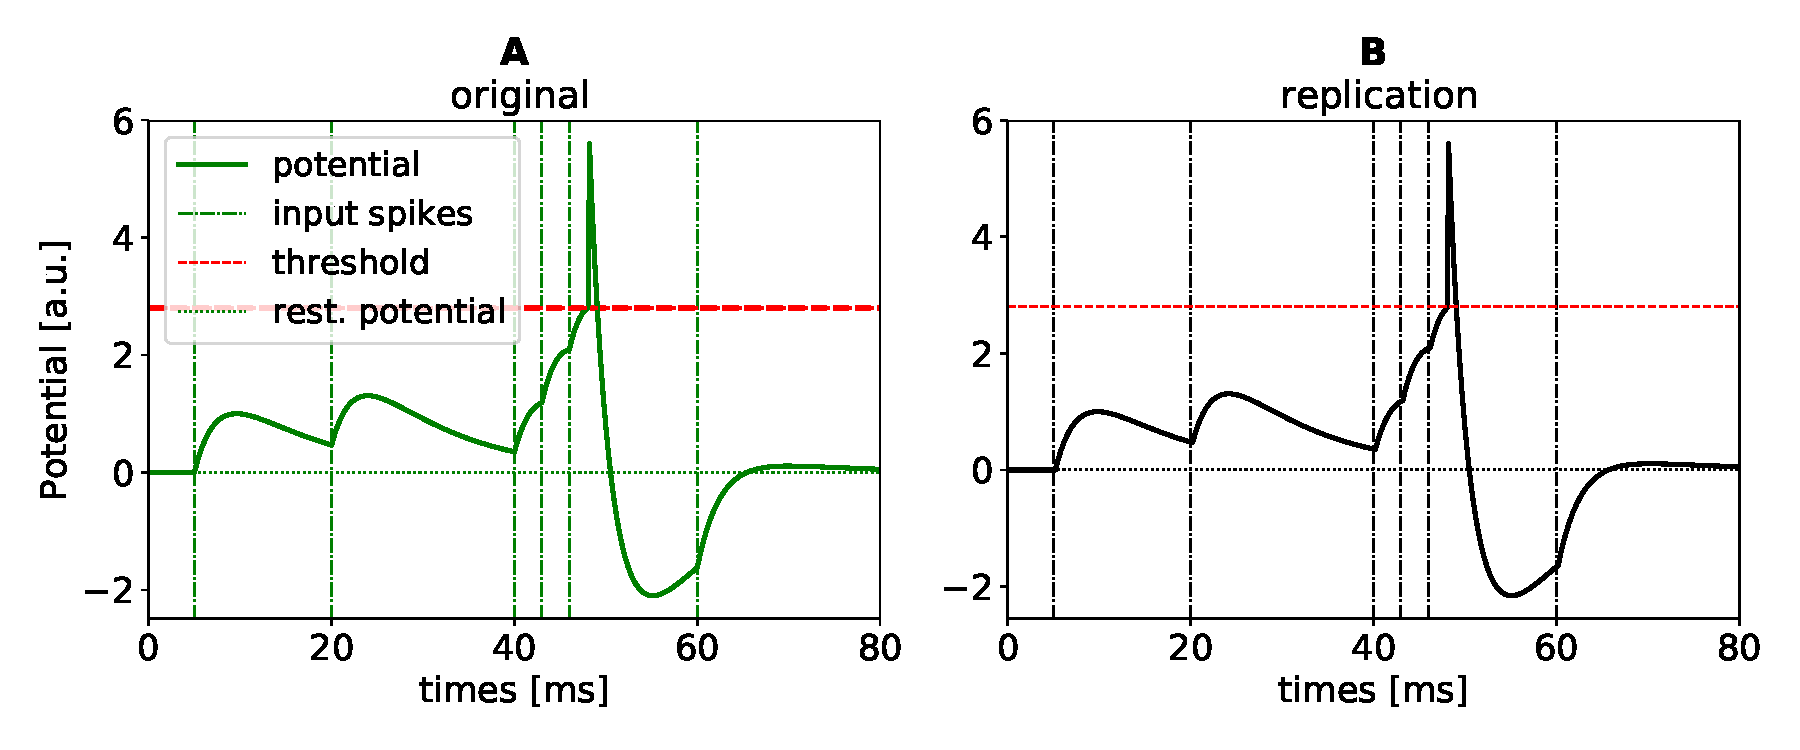
\includegraphics{figures/fig1_potentials.pdf}
\caption{Postsynaptic potential. The postsynaptic potential of the
replication implementation behaves the same as in the original study.
Both show the same EPSP shapes and the negative afterpotential after a
postsynaptic spike. \textbf{A}) The postsynaptic potential of the
original study was calculated using the equations given in the original
paper. \textbf{B}) The postsynaptic potential in the replication
implementation was calculated from the differential equations specified
in section \textbf{Leaky Integrate and Fire neuron}}\label{fig:pot}
\end{figure}

\subsection{Spike Timing Dependent
Plasticity}\label{spike-timing-dependent-plasticity}

For synaptic plasticity, the original study uses the reduced nearest
neighbor rule (RNN) \autocite{Morrison2008} - a more restrictive version
of the nearest neighbor (NN) STDP rule. In the standard NN rule, every
spike causes a weight change (with the amount depending on the timing of
the nearest spike), while for RNN a weight change only happens for the
first postsynaptic spike immediately following a presynaptic spike (or
vice versa). This means that for NN, there can be a series of
potentiations or depressions, whereas for RNN potentiations and
depressions strictly alternate.

A visualisation of three STDP rules is shown in Fig.~\ref{fig:stdp}: the
RNN, the standard NN and the all-to-all (ATA) rule, in which all pairs
of spikes are considered to calculate the weight change. A case is
considered in which the presynaptic neuron (the input neurons in this
study) spikes more often than the postsynaptic neuron (the output neuron
in this study), leading to synaptic weight decreases for ATA and NN, but
no visible net change under RNN (Fig.~\ref{fig:stdp} \textbf{C}).

\begin{figure}
\centering
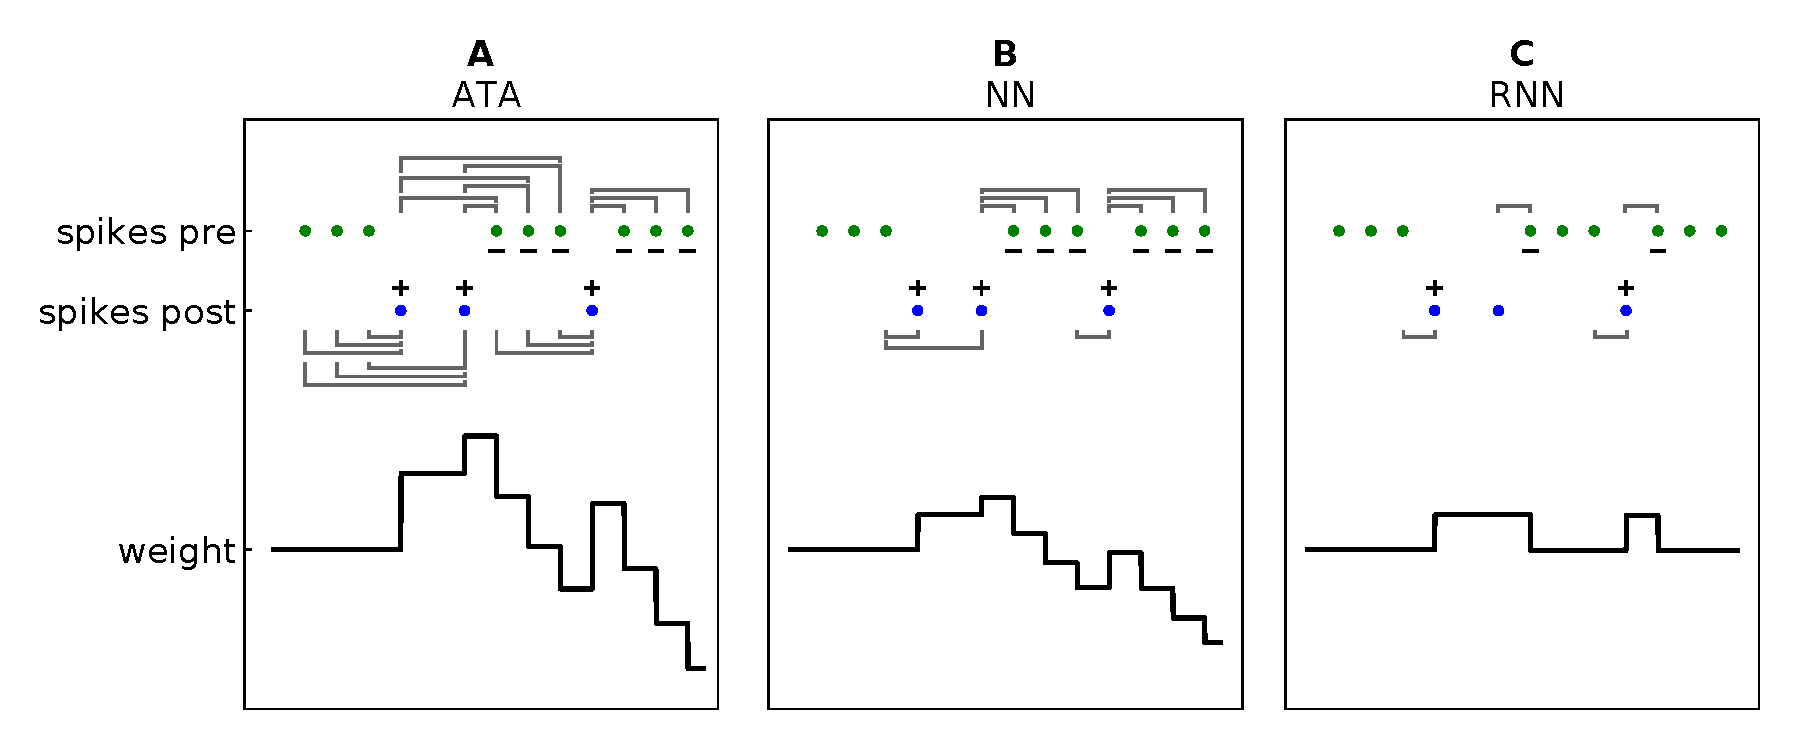
\includegraphics{figures/fig2_learningrules.pdf}
\caption{Effect of different learning rules on synaptic weight. We
compare the all-to-all (ATA, \textbf{A}), nearest neighbor (NN,
\textbf{B}), and reduced nearest neighbor (RNN, \textbf{C}) learning
rules for a case in which the presynaptic neuron (green dots) spikes
more often than the postsynaptic neuron (blue dots). Grey lines indicate
which spike pairs are taken into account for the calculation of the
synaptic weight change; the sign denotes a corresponding increase (+) or
decrease (-) in weight at that spike. The synaptic weight in ATA
(\textbf{A}) and NN (\textbf{B}) experience more weight changes and also
a net decrease in weight after only a few spikes. Under the RNN rule
(\textbf{C}), there are fewer changes and --- in this example --- no
visible net weight change.}\label{fig:stdp}
\end{figure}

\section{Results}\label{results}

The ability to find repeating patterns was reproduced in the replication
implementation. We could qualitatively reproduce all results of the
original paper and show the reproduced figures relevant to the model
behaviour: latency development (Fig.~\ref{fig:lat}), pattern specificity
after convergence (Fig.~\ref{fig:conv}), and robustness
(Fig.~\ref{fig:para}). In addition, we comment on some implementation
details that turned out to be relevant to replicating the original study
successfully: simulation time step, learning rule, EPSP shape.

\subsection{Pattern finding}\label{pattern-finding}

The latency measures the time of the output neuron spike relative to the
start of the pattern. If the spike occurs outside of the pattern
(\textgreater{}50 ms after the start of the pattern), the latency for
that spike is set to 0 as in the original paper.

In order to assess the time of pattern finding, we used the same spike
train (standard conditions) as input for both the original code and in
the replication implementation. The latency development looks similar in
both implementations (see Fig.~\ref{fig:lat}). The time until a stable
state arises is longer in the replication implementation (1400
discharges instead of 700 or 20 s instead of 13.5 s). This discrepancy
is due to the size of the discrete time steps used (see section
\textbf{Implementation details}).

\begin{figure}
\centering
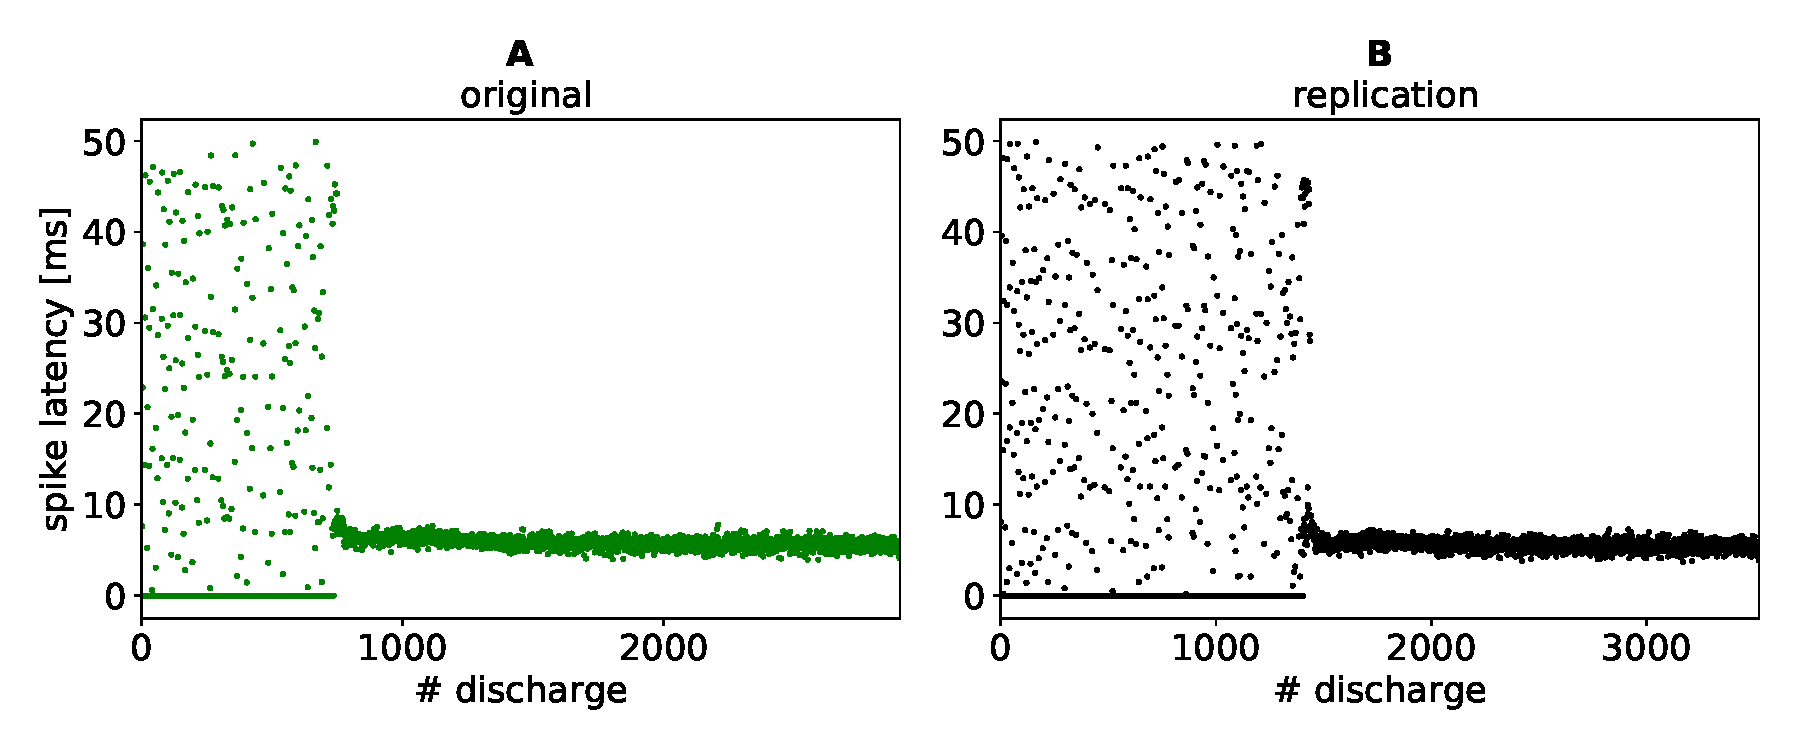
\includegraphics{figures/fig3_latency.pdf}
\caption{Latency. Comparing the latency development of the original
study (\textbf{A}) and the replication implementation (\textbf{B}). In
both implementations, the timing of the output spike in relation to the
start of the pattern (vertical axis, set to latency=0 if output spike
happens outside the pattern) is random at first, but becomes selective
after a few hundred discharges. From then on the postsynaptic neuron
always spikes only within the pattern (no spikes at latency = 0). The
number of discharges until this happens is smaller in the original paper
than in the replication implementation.}\label{fig:lat}
\end{figure}

At the end of the simulation, the synaptic weights that are maximally
potentiated (close to w\(_{max}\) = 1) belong exclusively to neurons
involved in the pattern, whereas weights from neurons not involved in
the pattern are depressed nearly completely (see Fig.~\ref{fig:conv}).
Neurons that spike at the beginning of the pattern are potentiated,
causing the postsynaptic neuron to spike at a low latency.

\begin{figure}
\centering
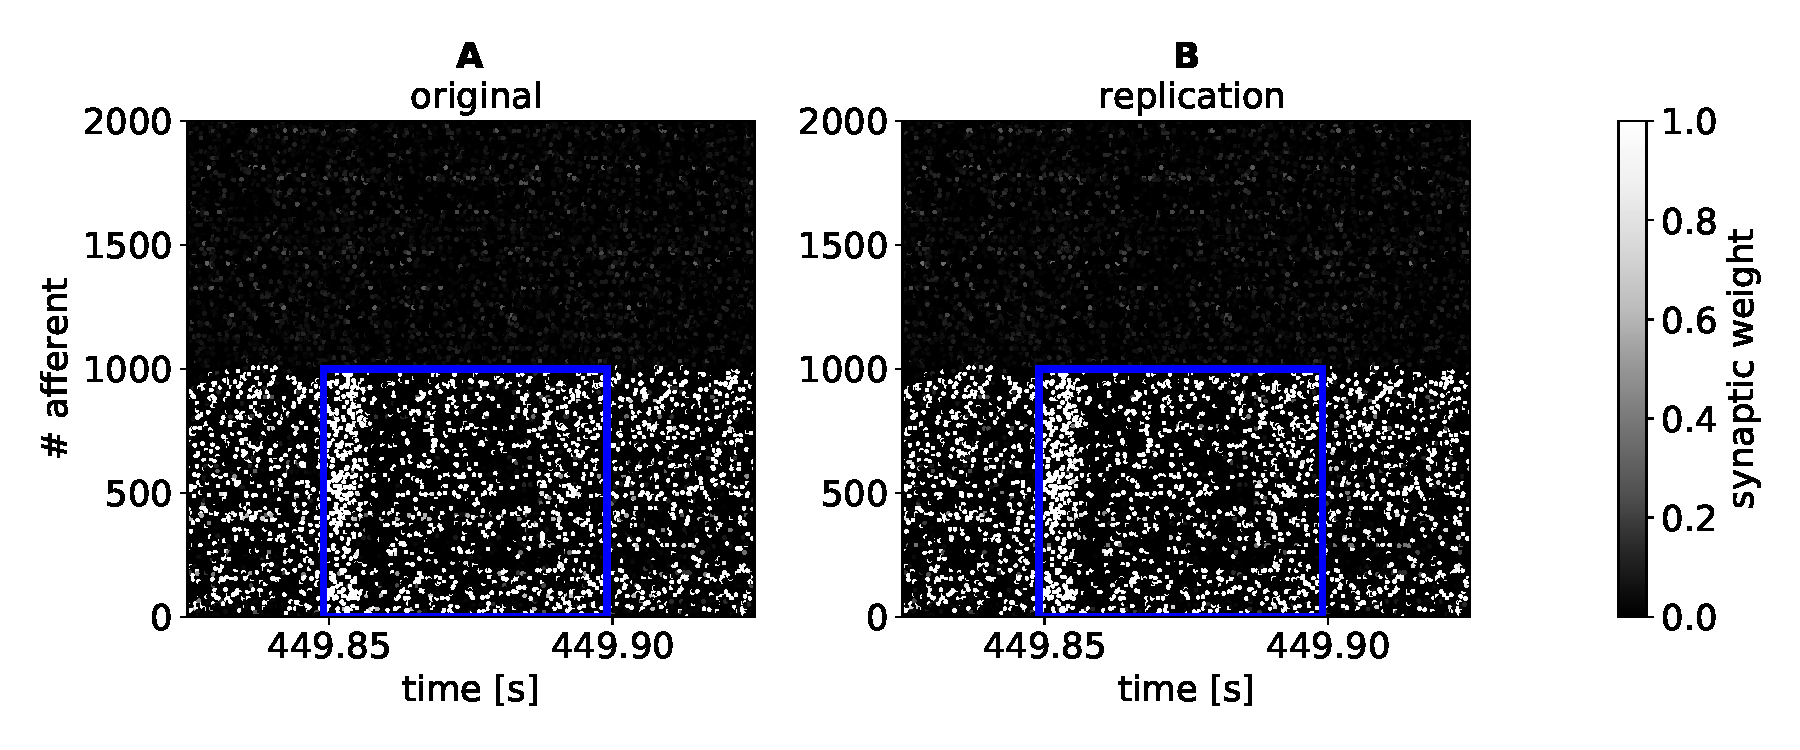
\includegraphics{figures/fig4_convergence.pdf}
\caption{Weights at converged state. This figure shows a raster plot of
the input spikes at the end of the simulation (converged state) with the
color of the dots indicating the synaptic weight. The final weights in
the converged state look very similar in the the original study
(\textbf{A)}) and the replication implementation (\textbf{B)}). Weights
from neurons not involved in the pattern are close to 0 (black, neurons
1000-1999), whereas weights from some neurons involved in the pattern
(neurons 0-999) are close to 1 (white, maximum value). The weights of
neurons that spike at the beginning of the pattern are nearly all close
to 1 and their added postsynaptic potentials cause a spike at the
beginning of the pattern (blue rectangle).}\label{fig:conv}
\end{figure}

Both latency development and the potentiation of only synaptic weights
of pattern neurons in the converged state were successfully reproduced
by the replication implementation.

\subsection{Robustness}\label{robustness}

Our simulations showed largely the same resilience to degradations as in
the original paper, but despite the very similar implementations, there
were some differences.

The replication implementation behaves the same as the original study
when subjected to different amounts of jitter (Fig.~\ref{fig:para}
\textbf{B}), various proportions of neurons involved in the pattern
(Fig.~\ref{fig:para} \textbf{C}), different initial weights
(Fig.~\ref{fig:para} \textbf{D}) and when a percentage of spikes within
the pattern are deleted (Fig.~\ref{fig:para} \textbf{E}).

\begin{figure}
\centering
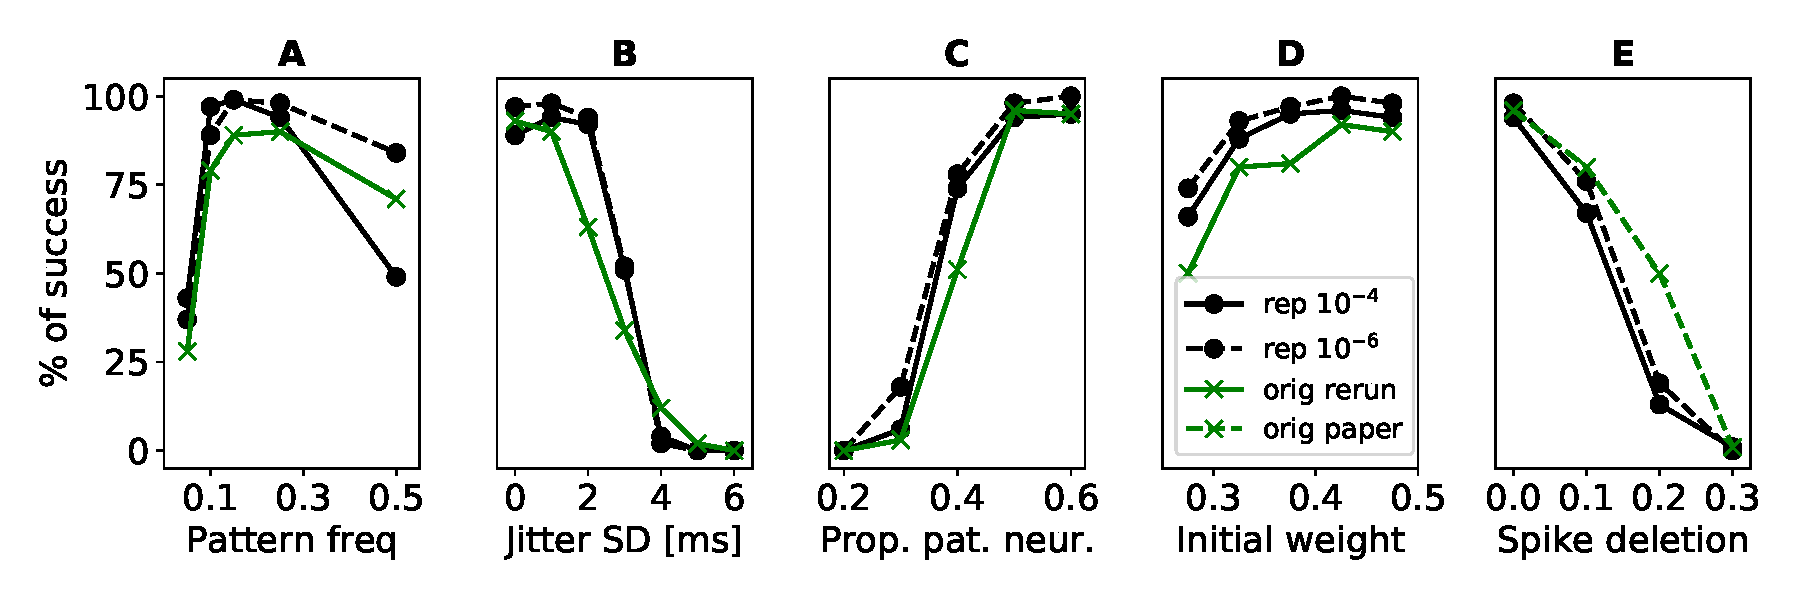
\includegraphics{figures/fig5_robustness.pdf}
\caption{Robustness. Pattern finding abilities of the system were tested
against different pattern presentation frequencies (\textbf{A}), jitter
(\textbf{B}), number of neurons spiking according to the pattern
(\textbf{C}), initial weights (\textbf{D}) and deletion of spikes in the
pattern (\textbf{E}). For each parameter combination 100 simulations
were run and the number of successful runs are reported as percentage of
success. The replication implementation was run at two different time
steps: 10\(^{-4}\) s (solid black lines) and 10\(^{-6}\) s (dashed black
lines). The results from the original study were calculated using the
source code provided (solid green lines in \textbf{A}, \textbf{B},
\textbf{C}, \textbf{D}) or estimated from the original publication
(dashed green line in \textbf{E}).}\label{fig:para}
\end{figure}

At a high pattern repetition frequency of 0.5 (Fig.~\ref{fig:para}
\textbf{A}), when the pattern is presented every 100 ms for 50 ms, the
performance of the replication differs from the original: at larger time
steps of 10\(^{-4}\) s the replication version does not perform as well
as the original, but shows good results at smaller time steps
(10\(^{-6}\) s).

\begin{figure}
\centering
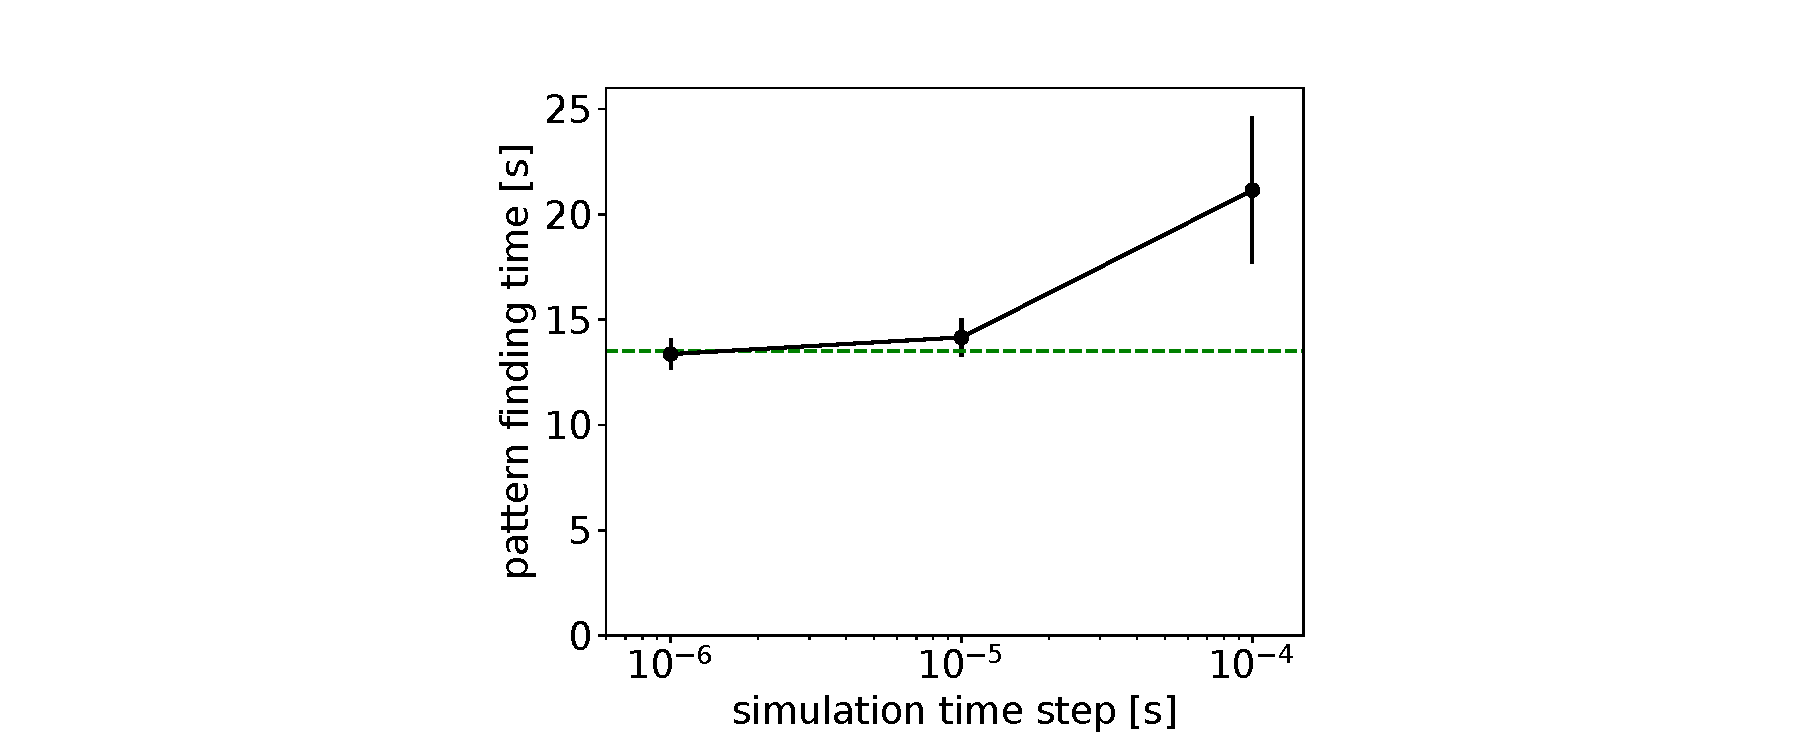
\includegraphics{figures/fig6_findtime.pdf}
\caption{Time until finding pattern. Using larger simulation time steps
leads to the pattern to be found later. The horizontal striped green
line is the reported time when the pattern is found by
\textcite{Masq2008}. Errorbars represent standard deviation from 100
successful runs.}\label{fig:find}
\end{figure}

\subsection{Implementation details}\label{implementation-details}

We noticed that small implementation details can affect the behaviour of
the network significantly. We summarised the relevant details in Table
tbl.~\ref{tbl:impl}.

\subsubsection{Simulation time step}\label{simulation-time-step}

In the standard parameter configuration, the time step chosen does not
have an effect on overall pattern finding success, as long as the time
step is less than or equal to 10\(^{-4}\) s. At larger time steps
(10\(^{-3}\) s), no specificity emerges. Instead there is a systematic
potentiation of all synaptic weights leading to very high firing rates
in the output neuron. In contrast, success rates are above 95\% for
10\(^{-4}\) s, 10\(^{-5}\) s, 10\(^{-6}\) s, and 10\(^{-7}\) s.

Although the success rate stays roughly the same, the time until the
pattern is found (defined as the time after which no output spikes
happen outside of the pattern) increases with larger time step size. An
example can be seen in Fig.~\ref{fig:lat}: the pattern is found after
about 700 output neuron spikes in the original publication (left) and
after about 1400 in the replication implementation (right) at a time
step of 10\(^{-4}\) s for the same input. At smaller times steps
(10\(^{-6}\) s), the pattern is found after about 700 discharges - the
same as in the original publication (Fig.~\ref{fig:find}).

\hypertarget{tbl:impl}{}
\begin{longtable}[]{@{}lrr@{}}
\caption{\label{tbl:impl}Implementation details }\tabularnewline
\toprule
& works & does not work\tabularnewline
\midrule
\endfirsthead
\toprule
& works & does not work\tabularnewline
\midrule
\endhead
simulation time step & continuous, discrete &\tabularnewline
time step size & \(\leq\) 10\(^{-4}\) s & \textgreater{} 10\(^{-4}\)
s\tabularnewline
learning rule & RNN & ATA, NN\tabularnewline
EPSP shape & kernel & immediate voltage increase\tabularnewline
\bottomrule
\end{longtable}

\subsubsection{Version of STDP learning
rule}\label{version-of-stdp-learning-rule}

The choice of learning rule is crucial for the pattern finding abilities
of the network. The RNN rule results in stable posystnaptic firing and
reliable finding of the pattern. The use of other learning rules does
not result in stable learning.

The spike trains used here involve neurons with a continuously high
firing rate in the input neurons (on average 64 Hz, min 30 Hz, max 90
Hz) and a significantly lower firing rate in the output neuron (63 Hz
initially, 5Hz after reaching specificity). This means that input
neurons fire often in the time between output neuron spikes. Therefore,
with any other than the reduced NN learning rule, the input neurons will
experience a decrease in weight a lot more often (every time an input
neuron spikes) than an increase in weight (every time the postsynaptic
neuron spikes). This leads to a strong overall depression of the
synaptic weights in the first few seconds of the simulation. With the
parameters specified in \textcite{Masq2008} and an ATA or a conventional
NN learning rule, the output neuron stops firing after a few seconds
because the output neuron voltage does not reach the voltage threshold
necessary to evoke an output neuron spike anymore (see
Fig.~\ref{fig:meanw}). In the case of the standard parameters, the
output neuron stops firing after less than one second. When no output
neuron spikes occur, learning cannot take place and no specificity can
emerge.

\begin{figure}
\centering
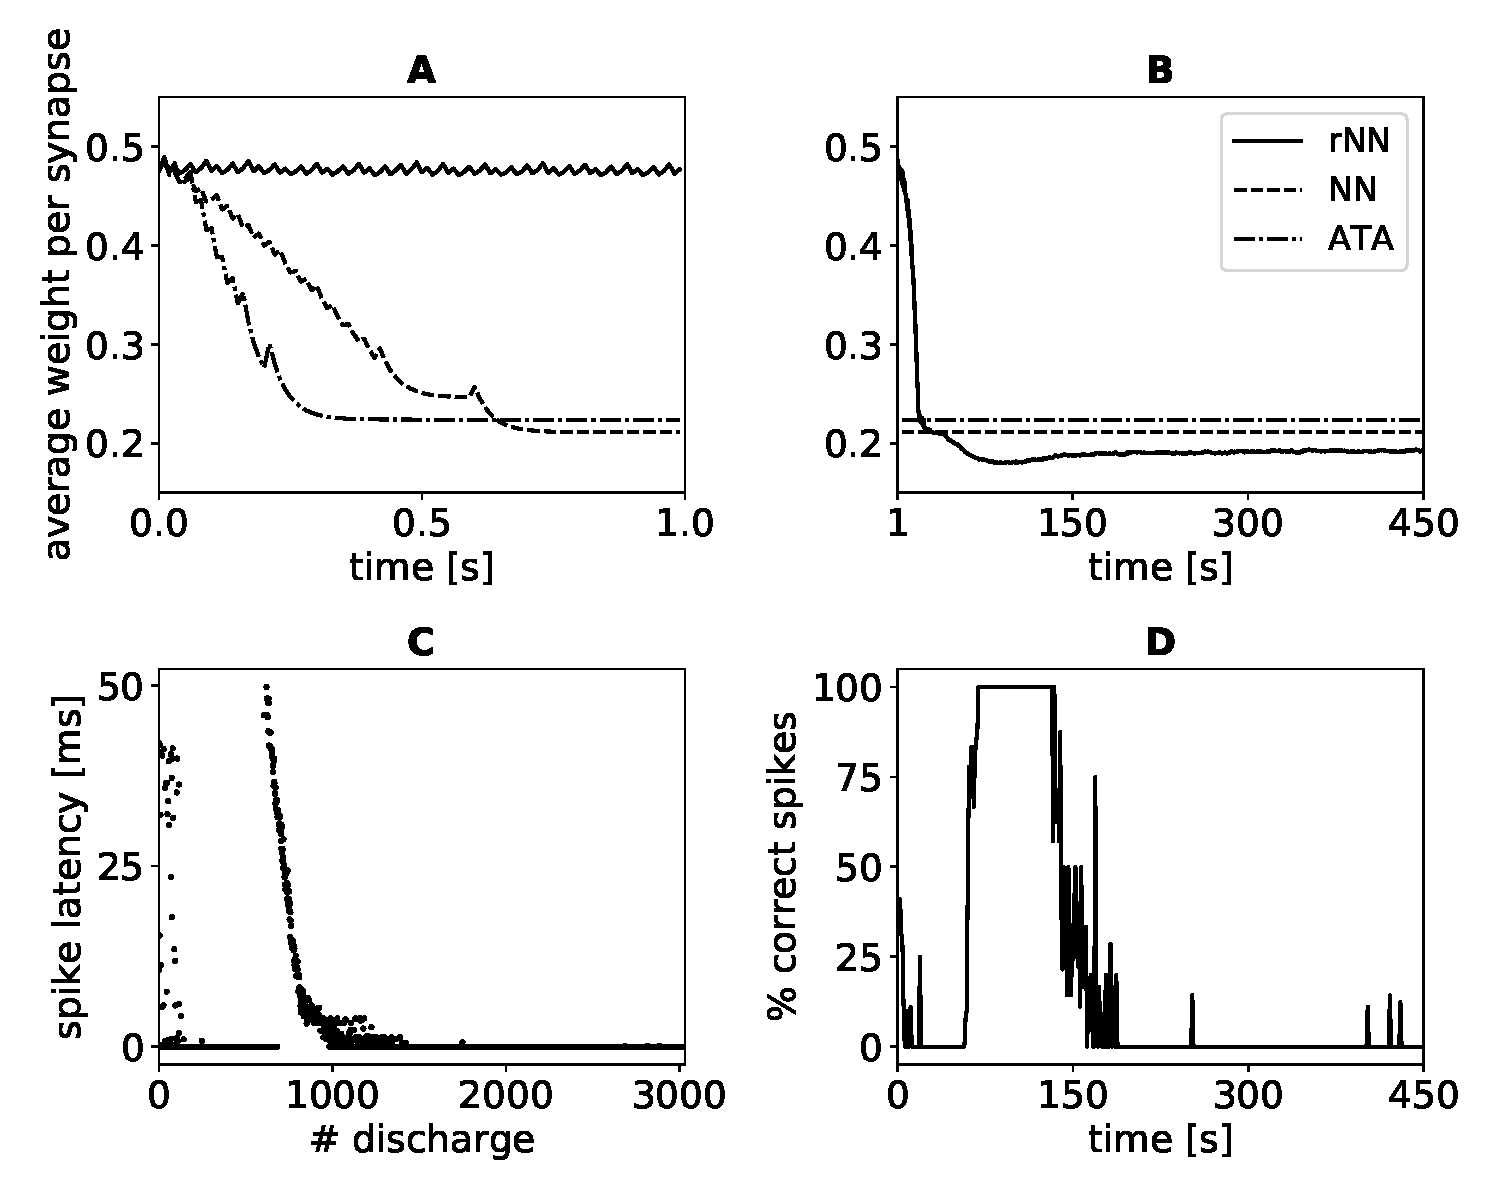
\includegraphics{figures/fig7_ata.pdf}
\caption{Effect of learning rules on synaptic weights. \textbf{A)} Both
the ATA and the NN rules lead to a very rapid depression of all synapses
leading to silence in the output neuron. \textbf{B)} In contrast, the
average weight of all neurons declines at a much slower rate for the RNN
rule. \textbf{C)} and \textbf{D)} When tweaking the ATA rule (increasing
\(a_{+}\) substantially) it is possible to achieve a behaviour that
resembles pattern finding. For a short amount of time the output neuron
becomes specific to the pattern, but loses this ability again and does
not regain it.}\label{fig:meanw}
\end{figure}

In the case of an ATA learning rule, a behaviour resembling pattern
finding can be evoked under the right circumstances: reducing the
learning rate by a factor of 5 and increasing the value of \(a_{+}\)
(the maximum weight increase) to double the value of \(a_{-}\) (the
maximum weight decrease). This setup works because the large amount of
depression (on every input spike) is counteracted by large potentiation
(due to the increased \(a_{+}\)). In such runs, the output neuron will
correctly reach specificity and trace back through the latency, but then
starts firing outside of the pattern again. This system is not stable
since the ATA rule leads to ``too much learning'' as the synaptic
weights change after every single spike. A further reduction in the
learning rule will not result in pattern specificity at all.

We were unable to find parameters for the standard NN learning rule that
allowed for pattern finding, despite this rule exhibiting slower
learning when compared to the ATA rule. In the case of both the ATA and
NN learning rules, it seems likely that stable pattern finding relies on
a precise balance of \(a_{+}\) and \(a_{-}\), with runaway potentiation
or depression likely if the balance is wrong. By contrast, the RNN rule
is automatically balanced and is not subject to this issue.

\subsubsection{\texorpdfstring{Effect of learning rule at
\(\Delta t=0\)}{Effect of learning rule at \textbackslash{}Delta t=0}}\label{effect-of-learning-rule-at-delta-t0}

The spike times of the output neuron are slightly different in the
original study and the replication. In the original study spike times of
the input and output neurons are not restricted to fixed multiples of
the timestep, so it is extremely unlikely that two neurons will spike at
the same time. In Brian, the output neuron spikes at the beginning of a
time step and will therefore happen in the same time bin as some input
neuron spikes leading to a time difference between the spikes of
\(\Delta t=0\) where the STDP rule is undefined. Brian treats all of the
input neuron spikes in this time bin as if they happened just before the
output neuron spike (\(\Delta t<0\), due to the scheduling of events in
Brian) and will therefore increase all those weights instead of
increasing some and decreasing others. This higher number of
potentiations makes it more difficult for the system to systematically
depress unimportant weights in order to become selective to the pattern.

If the learning rule is modified so that the change in synaptic weight
reflects that on average half the input neurons spike before the output
neuron and the other half afterwards (by adding the mean of LTP and LTD
traces), the pattern is found earlier, at around 17 s or 850 spikes (for
a time step of \(10^{-4}s\)) which is close to the performance for
smaller time steps (\(10^{-6}s\)) and the original paper (both 14 s or
700 spikes). This modified learning rule was only used to determine the
time until finding (Fig.~\ref{fig:find}) because it differs from the
implementation used in the majority of modelling papers.

This difficulty to depress non-relevant input neurons is the reason for
the lower success rate at a high pattern presentation frequency at large
time steps (\(10^{-4}\) s) as seen in Fig.~\ref{fig:para} \textbf{A}).
The time until the pattern is found during this condition is notably
longer (\textgreater{}30 s instead of 20 s) and points towards towards
the difficulties of the system to properly depress the synaptic weights
of the non-pattern neurons.

\subsubsection{EPSP shape}\label{epsp-shape}

The kernels used in the original study simulate a gradual increase of
the postsynaptic neuron voltage as can be seen in Fig.~\ref{fig:pot}.
Other studies sometimes also model the effect of the presynaptic spike
as an immediate jump in postsynaptic voltage instead of that gradual
increase. In this system, using an immediate increase in postsynaptic
voltage does not lead to stable pattern finding. This might have to to
with the fact that the kernel shape and the immediate increase exhibit
slightly different spike times as seen in Fig.~\ref{fig:epsps}.

\begin{figure}
\centering
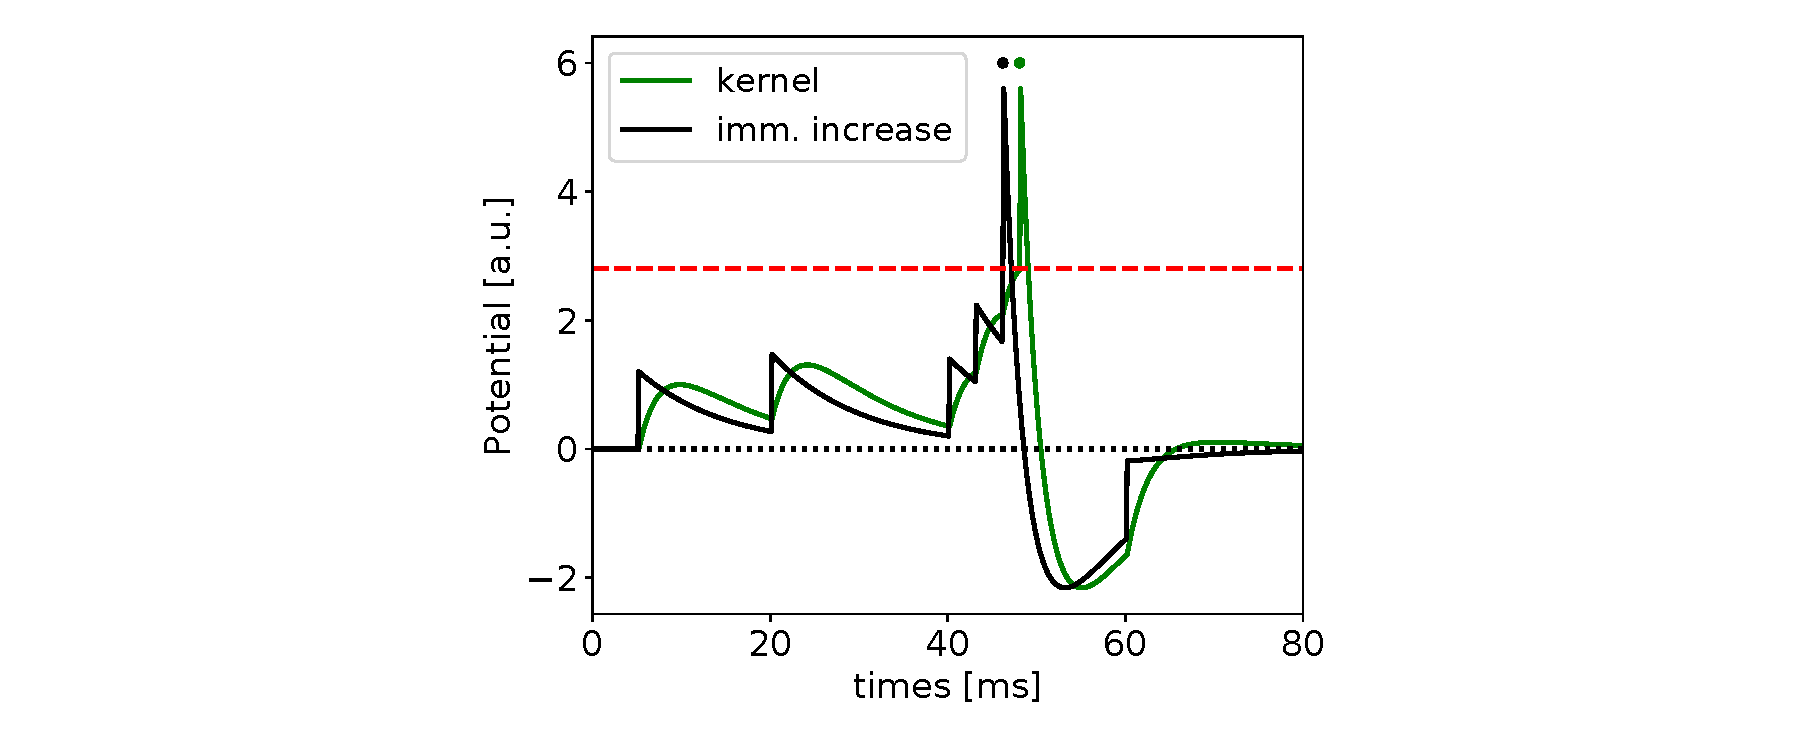
\includegraphics{figures/fig8_kernel_vs_imm.pdf}
\caption{Choice of EPSP. For the same presynaptic spikes, the
postsynaptic voltage behaves similarly, but the postsynaptic spike time
is slightly different (green and black dots).}\label{fig:epsps}
\end{figure}

When modelling the immediate voltage increase, one needs to set the
magnitude of the voltage increase (for Fig.~\ref{fig:epsps} \(\Delta u\)
was set to 1.2). It is very difficult to find the \(\Delta u\) that
corresponds to the same amount of voltage increase from the kernel. If
the value of \(\Delta u\) is too small, then the output neuron stops
firing after a short period of time without having gained specificity
for the pattern. If the value for \(\Delta u\) is too high all input
neurons are potentiated and the output firing rate rockets. For the
scope of this paper, no value for \(\Delta u\) was found to induce a
stable pattern finding behaviour.

\section{Conclusion}\label{conclusion}

We could successfully replicate the results from \textcite{Masq2008} - a
neuron with STDP synapses could reliably find a repeating spike pattern
and afterwards spike only when the pattern is presented. The time when
the pattern is found depends on the time step size chosen for the
simulation, whereas the success of reliably finding the pattern requires
the precise learning rule and the shape of the EPSPs. Reproducing the
paper was made easy by the fact that simulation parameters were stated
in the text and the source code was shared by the authors of the paper
on request.

\textbf{Introducing discrete time steps.} To run the simulations in
Brian, we introduced discrete time steps. This did not affect pattern
finding abilities (as long as the time steps are \(10^{-4}\) s or
smaller), but it did increase the time until a pattern was found for
large time steps (\(10^{-4}\) s), but not for small time steps
(\(10^{-6}\) s).

We verified that the delay in pattern finding did not stem from either
the deletion of some input spikes (to avoid input neurons spiking twice
in one time step) or the spike timing being at the start of each 0.1 ms
time bin. When we fed those modified input spikes to the original
implementation, the timing of finding the pattern was not affected. The
delay therefore stems from forcing the output neuron to spike at the
beginning of a time step and the associated consequences for STDP
learning.

Running the simulations using discrete time steps does not negatively
impact pattern finding abilities, but delays pattern finding for large
time steps due to a larger number of potentiations.

\textbf{Choice of learning rule.} The learning rule used is one specific
version of a NN STDP rule, which was not clearly stated in the original
article. The comparison with other learning rules shows that the use of
this particular learning rule enables the pattern finding behaviour.

The usage of the RNN rule has two interesting consequences. Firstly, it
slows down the rate of synaptic weight change, since it considers fewer
spike-spike interactions than other learning rules. This slows down
overall weight changes significantly and gives the system more time to
learn the spike sequences of the pattern. Neurons that spike together
during the pattern will experience similar weight changes more often
than non-pattern neurons. Over the course of hundreds of output neuron
spikes - until pattern specificity arises - these synchronised weight
changes lead to higher synaptic weights for the pattern neurons than for
the non-pattern neurons.

Secondly, for this particular input the restrictions of the RNN STDP
rule lead to the weights alternating between increase and decrease. The
stabilising effect of this is most clear during the converged phase. The
output neuron only spikes when a pattern is presented more or less at
the same latency. The input neurons (which are forced to spike at least
once every 50 ms) reliably spike at least once before or after or both.
In the latter case the input neurons will always experience the same
increase or decrease in synaptic weight per output neuron spike
disregarding small changes due to jitter and noise. If the input neuron
only spikes once per pattern, then either the increase or decrease of
weight will be nearly constant whereas the respective decrease or
increase in weight will be random. On average the weights of all input
neurons will slowly increase to 1 or decrease to 0 over time, resulting
in a very stable system.

\textbf{Choice of EPSP shape.} It seems to be essential to use a kernel
EPSP shape since using immediate voltage increases as the effect of an
input neuron spike does not lead to learning of the pattern. This might
be due to the difficulty in finding the correct parameters that create
an equivalent voltage increase. It seems likely that the EPSP shape is
responsible for the decrease in success, since small changes in output
neuron spike times also occur when using different time step sizes and
do not affect pattern finding abilities under standard conditions.

{\sffamily \small
  \printbibliography[title=References]
}
\end{document}
